\section{Evaluation Methodology}
\label{sec:evaluation:methodology}

% Talk about standard evaluation methodology and its drawbacks
Even though activity recognition is very diverse in terms of sensor approaches and algorithmic choices, evaluation is usually carried out applying a very well known methodology which can be summarised in the following steps:

\begin{enumerate}
 \item Choose a target environment and deploy sensors to acquire and process information about human activities. 
 \item Select a group of persons who can perform target activities in the prepared environment.
 \item Select a dataset labelling system so datasets generated by users can be used as a ground truth, both for the activity recognition system and the evaluation process.
 \item Run experiments with users and label obtained activity datasets.
 \item Use the same datasets to test the activity recognition system and store the labels produced by it.
 \item Compare the labels of the activity recognition system with the ground truth using appropriate metrics.
\end{enumerate}

% Insert a diagram that shows the standard methodology

Each of the enumerated steps may vary depending on the activity recognition approach and the available resources. The described methodology, which will be called \textit{standard methodology} for the rest of the paper, is the reference for any group working on human activity recognition.

Nevertheless, there are some problems that make very difficult to implement the standard methodology. For instance, (i) it is not always possible to own an environment and install sensors and processing systems, due to economic reasons, (ii) running experiments with human beings imply ethical and legal issues that can slow down the research process or sometimes make it impossible, (iii) dataset labelling systems are not perfect, since most of them rely on users' memory or discipline to annotate every activity carried out, and (iv) regulatory limitations on the use of human subjects prohibit the collection of extensive datasets that can test all scenarios and theories under all circumstances. 

There are several research groups that share the datasets they obtain in their pervasive environments, following different variants of the standard methodology. A Wiki Page called BoxLab\footnote{http://boxlab.wikispaces.com/List+of+Home+Datasets} contains a detailed list of public datasets collected in home environments. It contains a description of deployed sensors, whether it is an annotated dataset and the availability of the dataset. Those public datasets can be a very good alternative for those research groups which cannot run their own experiments. Furthermore, public datasets can also be used for benchmarking different activity recognition systems.

%This paper presents a novel evaluation methodology to overcome the enumerated problems. The methodology has been named \textit{hybrid} because it combines real users' inputs and simulation tools. The key idea is to circulate surveys among target users with the objective of capturing how they perform certain activities of daily living. Using the information collected by surveys, individual scripts are prepared, which are then processed by a synthetic dataset generator tool to simulate arbitrary number of days and generate perfectly labelled datasets of activities. To get as close as possible to real world settings, the synthetic dataset generator uses probabilistic sensor noise models and probabilistic time lapses.

% Present the hybrid methodology and show its need and benefits

\subsection{Analysis of the Viability of the Standard Methodology for the Extended Activity Model Learning System}

To evaluate properly the EAM learning system, activity datasets that fulfil several conditions are needed. Namely:

\begin{enumerate}
 \item Contain a lot of samples of different activities to enable a proper learning process.
 \item Sensor activations must be labelled in order to provide a solid ground truth.
 \item Specific objects used for activities have to be monitored (dense sensing scenario).
 \item At least some of the activities have to be performed in varied ways to see whether the presented learning process can capture all those variations.
 \item Several users are needed as the approach aims at capturing concrete activity models for concrete users. 
\end{enumerate}

Following the standard methodology to generate such datasets implies a high-cost process with many ethical and legal constraints regarding the use of people for experiments. That cost, both economical and time cost, could not be assumed during the development of the current dissertation. Due to this limitation, public dataset repositories were analysed carefully to find an appropriate dataset.

Unfortunately, datasets that meet all the enumerated conditions could not be found in those public repositories. Some datasets used different activity monitoring approaches, such as vision- and wearable-based monitoring. Some other datasets could be used for the dense sensing scenario since they monitor specific objects, but activities are performed from a list where no variations can be found. Yet other datasets are more focused on monitoring the contextual information, rather than concrete user-object interactions.

As Helal et al. state in their paper \cite{Helal2011}:

\blockquote{\textit{Access to meaningful collections of sensory data is one of the major impediments in human activity recognition research. Researchers often need data to evaluate the viability of their models and algorithms. But useful sensory data from real world deployments of pervasive spaces are very scarce. This is due to the significant cost and elaborate groundwork needed to create actual spaces. Additionally, human subjects are not easy to find and recruit. Even in real deployments, human subjects cannot be used extensively to test all scenarios and verify multitudes of theories. Rather, human subjects are used to validate the most basic aspects of the pervasive space and its applications, leaving many questions unanswered and theories unverified.}}

This is the case of the presented approach for EAM learning. It turns out that there cannot be found datasets from real pervasive environments to verify the exposed theory. However, Helal et al. propose a solution to this problem in the same paper \cite{Helal2011}:

\blockquote{\textit{It is thus necessary to develop alternative and practical approaches to studying human activity recognition. Powerful and realistic simulation tools could be used to support the growing demand for test data. Simulations enable researchers to create focused synthetic replications of important events and activities under study. It can be easily changed and refined allowing researchers efficiently to experiment, analyze and fine-tune their models and associated algorithms. Simulation also allows a wider community of researchers to engage and collaborate to solve a specific problem. Hence, a design based on preliminary simulation studies would most likely to be a more robust and inclusive design. Also, a simulation model that mimics an existing real world pervasive space is most likely to answer more questions (and generate much more data) than the target actual space.}}

Following those ideas simulation tools have already been used for activity recognition. For example,   Okeyo et al. use a synthetic data generator tool to simulate time intervals between sensor activations \cite{Okeyo2012a}. Their research is focused on sensor data stream segmentation, so the tool generates varying patterns of sensor activations in order to verify their approach. Liao et al. combine simulation tools and real data for activity recognition in \cite{Liao2006}. A more elaborated simulator has been developed by Bruneau et al. in \cite{Bruneau2009}: DiaSim. The DiaSim simulator executes pervasive computing applications by creating an emulation layer and developing simulation logic using a programming framework. However, it is more focused on simulating applications such as fire situations, intrusions, etc. to identify potential conflicts. In consequence, DiaSim cannot be directly applied to activity recognition. Finally, Helal et al. propose to develop powerful and realistic simulation tools to study human activity recognition. They develop a simulator called \textit{Persim}, which has been enhanced in the new version \textit{Persim-3D} \cite{Helal2012}. Persim is an event driven simulator of human activities in pervasive spaces. Persim is capable of capturing elements of space, sensors, behaviours (activities), and their inter-relationships. Persim is becoming a very complete simulator tool for activity recognition in pervasive environments. However, it is still in development and one of the main limitations is that it does not provide a way to model realistically human behaviour. Authors have already identified this limitation and they are currently working on programming by demonstration approaches to overcome the problem.

As it can be seen in the literature review done in the paragraph above, simulation tools can be used for activity recognition, since they provide accurate enough datasets to verify some theories. However, none of the references given above specify a concrete methodology to use simulators to evaluate activity recognition approaches. There is no information about how activities should be defined, how different users can be modelled, sensor error models, etc. which are key issues when using a simulator. Therefore, there is a lack of a sound methodology that addresses all those issues. 

\subsection{Hybrid Evaluation Methodology Approach}
\label{subsec:evaluation:hybrid}

\begin{comment}
 - Describe target scenario: dense sensing, single user - single activity
 - Explain in detail the steps: survey, script writing, sensor modelling, synthetic dataset generator 
\end{comment}

The hybrid evaluation methodology has been specially designed for activity recognition systems which assume the dense sensing paradigm (see constraint \ref{cons-dense}). Even though the methodology itself is not limited to concrete scenarios, the implementation presented in this document works for single user - single activity scenarios, i.e. only one user is considered and concurrent or interleaved activities are not taken into account (see constraint \ref{cons-single}). 

The methodology has been named hybrid because it combines real users’ inputs and simulation tools. The key idea is to circulate surveys among target users with the objective of capturing how they perform certain activities of daily living. Additionally, users are also requested to describe how their days are in terms of defined activities. For example, a user might make a coffee and brush teeth in week days between 7:00 and 7:30 AM. So the aim of those surveys is to model real human behaviour, covering one of the major weaknesses of simulation-based evaluation methodologies. Using the information collected by surveys, individual scripts are prepared, which are then processed by a synthetic dataset generator tool to simulate arbitrary number of days and generate perfectly labelled datasets of activities. To get as close as possible to real world settings, the synthetic dataset generator uses probabilistic sensor noise models and probabilistic time lapses.

Based on those constraints and ideas, the proposed hybrid evaluation methodology has the following steps (see Figure \ref{fig-methodology}):

\begin{enumerate}
 \item Design activity surveys: to capture how users perform activities and model their behaviour, a proper survey has to be designed. A detailed explanation of how surveys are designed for this dissertation can be found in Section \ref{subsubsec:evaluation:survey}.
 \item Select target users: depending on the objectives of the research, several user groups can be selected. For example, if the system aims at providing help to elderly people, selecting members of that target group is recommended.
 \item Distribute surveys among target users: a suitable way to distribute surveys has to be used, which guarantees users' anonymity. The distribution method can also be influenced by target users. For example, using web-based surveys can be a bad idea if surveys are directed to elderly people, who can be unfamiliar with those technologies. Personal interviews may be a good alternative for those cases.
 \item Translate surveys to scripts: this step is critical. Appropriate criteria have to be adopted to translate the answers obtained from surveys to scripts for the synthetic dataset generator - or any other simulator -. It is very important not to alter or lose the information provided by users.
 \item Model sensor noise: sensor noise has to be modelled in order to achieve realistic activity datasets. Real sensors are not perfect and depending on their technological base, error models have to be provided.
 \item Run synthetic dataset generator: using the scripts obtained from surveys and sensor error models, the synthetic dataset generator is executed. The output of the tool is a labelled activity dataset which will serve as the ground truth for evaluation.
 \item Develop the activity modelling and/or recognition system: researchers have to develop the activity modelling and/or recognition system in order to be tested. Notice that datasets generated by the synthetic dataset generator can also be used in this step, specially for data-driven approaches.
 \item Compare results: finally, the results obtained by the activity modelling and/or recognition system have to be compared with the ground truth, using appropriate metrics.
\end{enumerate}

\begin{figure}[htbp]
\centering
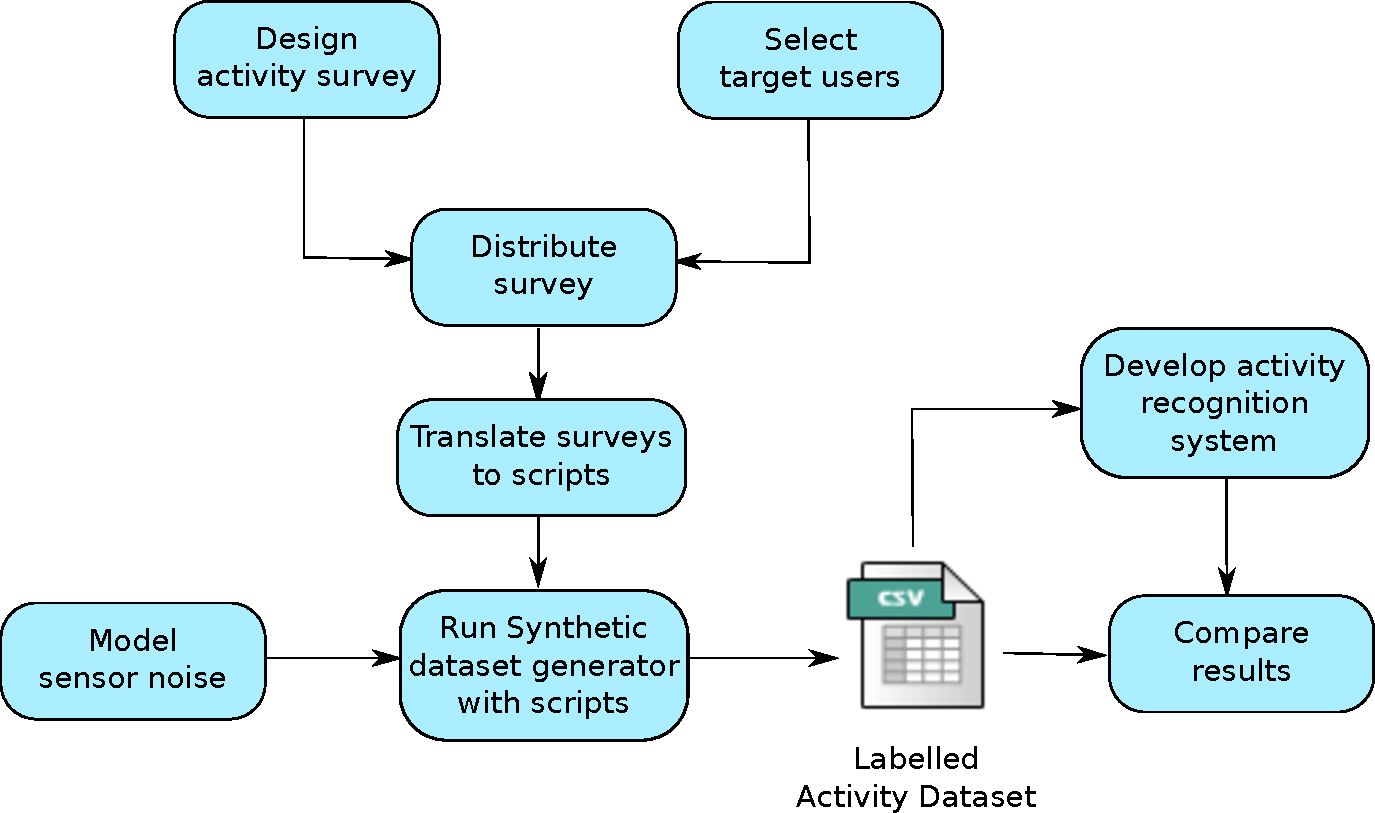
\includegraphics[width=\textwidth]{hybrid_methodology.pdf}
    \caption{The hybrid evaluation methodology steps depicted in a flowchart.}
    \label{fig-methodology}
\end{figure}

\subsubsection{Survey for Activities of Daily Living}
\label{subsubsec:evaluation:survey}
\begin{comment}
 - Explain each of the questions of the survey
 - Show a screenshot and provide the link to the Google Form
 - Google Forms guarantee users' anonymity
 - Explain survey-script translation criteria
\end{comment}

One of the main advantages of considering dense sensing scenarios is that activities are described in terms of the objects which have been used to perform that activity. Furthermore, as only sensor activations (and not de-activations) are important for the approach (see definition \ref{def-sa}), to model an activity, it is enough to know which objects are used by the user and the order of usage of those objects. This information is easy to obtain in a survey and will be named \textbf{activity model}.

\begin{defn}[Activity model]
\label{def-act-model}
 An activity model is a sequence of objects used by a user to perform an activity. A user might provide more than one activity model per defined activity, because the same activity can be performed in several ways. Activity models also provide a typical duration given by the user.
\end{defn}

On the other hand, to model human behaviour appropriately, acquiring activity models is not enough. It is very important to know what activities are performed by a concrete user in a daily basis, alongside with the time slots and time lapses between contiguous activities. 

\begin{defn}[Behaviour model]
\label{def-behaviour}
 A behaviour model is a sequence of activities with associated time slots and time lapses. A user might provide several behaviour models, as every day can be different in terms of performed activities and times.
\end{defn}

The main objective of the survey is to obtain activity and behaviour models from target users. Hence, the survey for activities of daily living has two main parts. The first part is devoted to capture what activities are performed in different days, i.e. behaviour models. The second part, on the other hand, asks users about how they perform those activities based on user-object interactions, i.e. activity models. The concrete survey used for the experiments carried out in this dissertation can be found in the web\footnote{http://goo.gl/etCNyi}. 

As it can be seen in Figure \ref{fig-survey-1}, the survey begins with a brief explanation for target users, where the aims of the survey are stated and the target activities are presented. In this case, target activities are seven: make a coffee, make a chocolate, make pasta, brush teeth, watch television, wash hands and read a book. Afterwards, under the heading of ``Day Description'', users are asked to describe their week days in terms of activities. They are expected to provide information about time slots and activity sequences performed in those time slots. Users are also asked to provide time relations between two consecutive activities. For example, between 7:00 and 7:30 AM a user might make a coffee and ten minutes later might brush teeth. This first part has been designed to obtain behaviour models for target users.

\begin{figure}[htbp]
\centering
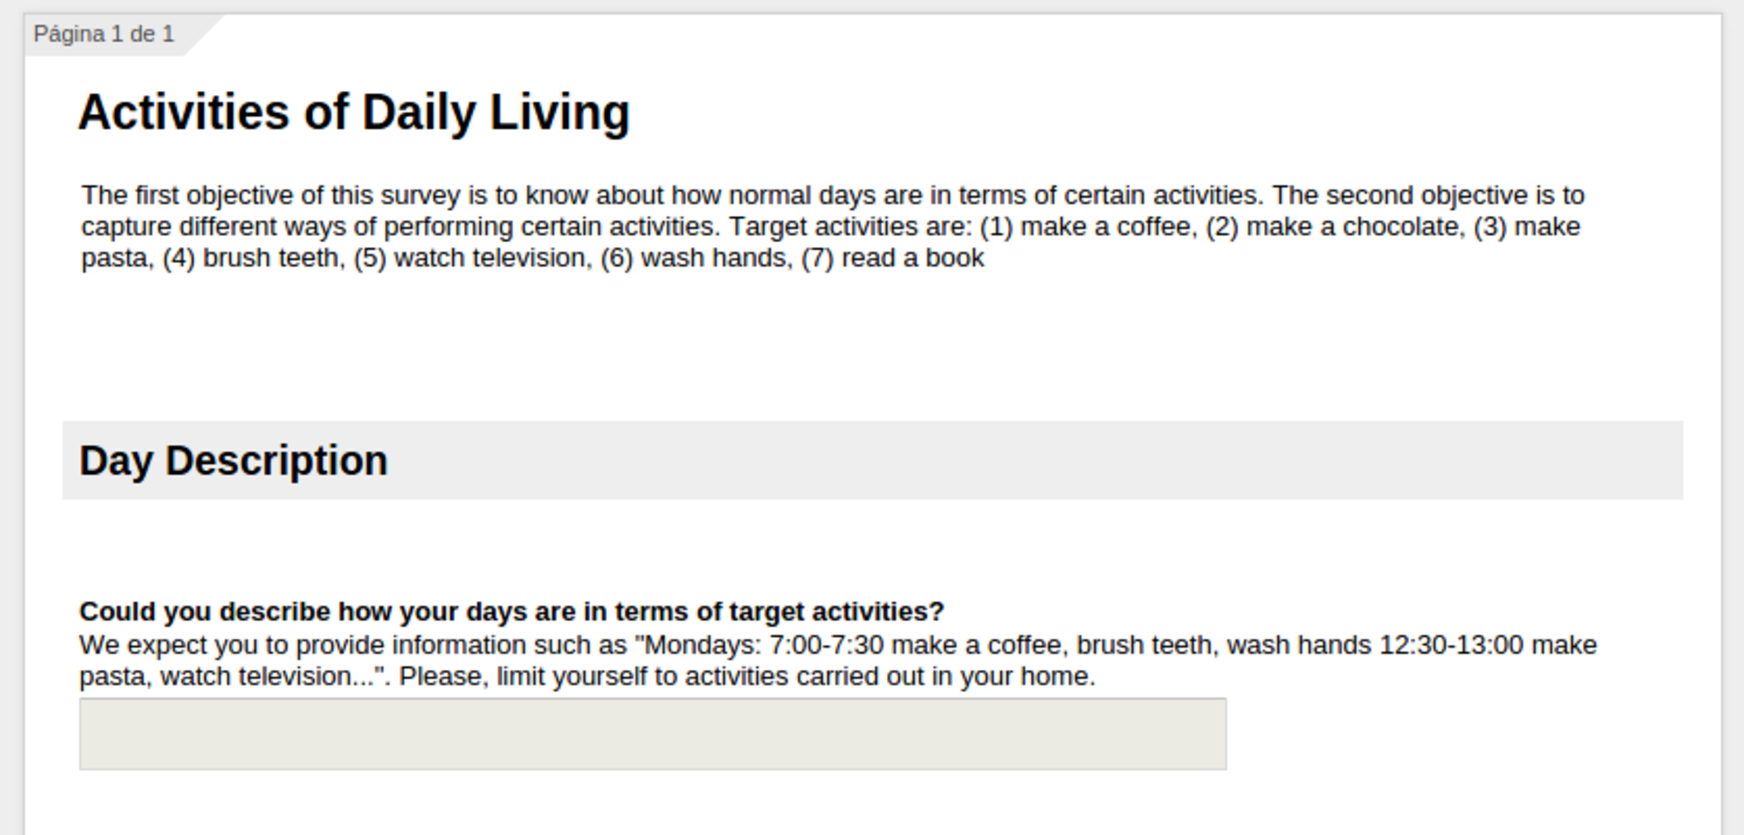
\includegraphics[width=\textwidth]{adl_survey_part1.pdf}
    \caption{The first part of the survey. A small introduction can be found where the aim of the survey is explained, continuing with the behaviour model part.}
    \label{fig-survey-1}
\end{figure}

The second part of the survey is longer. Target activities are presented one by one. For each activity, several questions are asked to users, to capture the locations of activities, the ways activities are performed, the objects used for each activity, a description of how those objects are used and typical duration estimations. An example of those questions can be found in Figure \ref{fig-survey-2} for the activity MakeCoffee.

\begin{figure}[htbp]
\centering
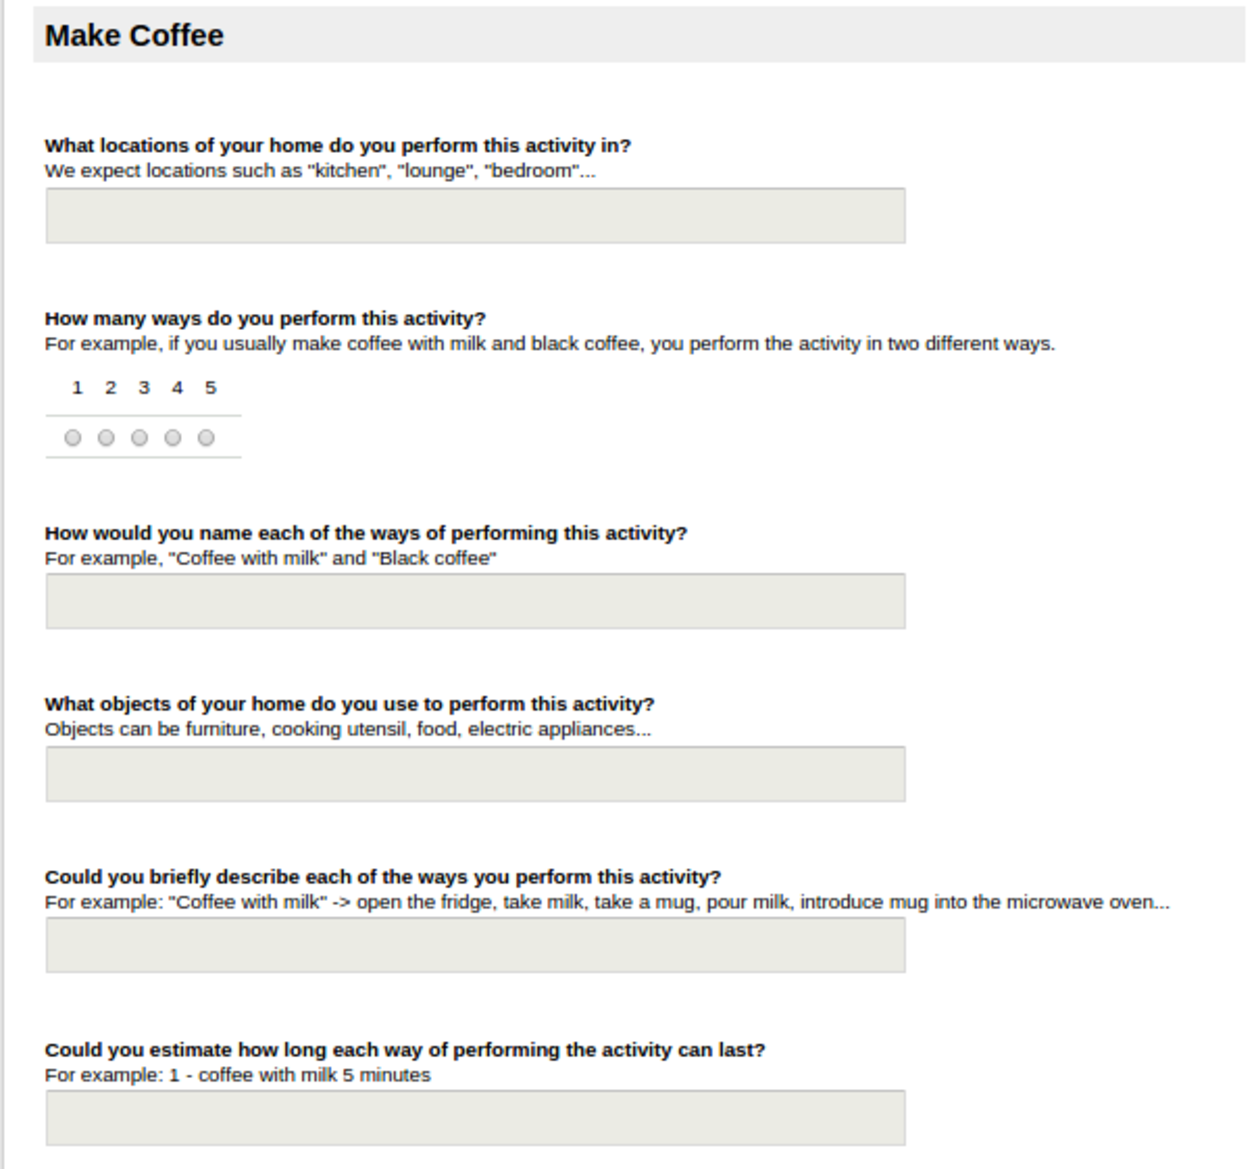
\includegraphics[width=\textwidth]{adl_survey_part2.pdf}
    \caption{The questions of the survey to capture the activity model of MakeCoffee.}
    \label{fig-survey-2}
\end{figure}

As Figure \ref{fig-survey-2} shows six questions are asked per activity. The first question is to know where the activity is performed by the user. As stated in the brief explanation under the question, expected locations are home locations such as kitchen, lounge, etc. Each activity may be performed in several locations, in concordance with the context knowledge model shown in Figure \ref{fig-context-json}. Notice also that expected locations fulfil with the location definition given in definition \ref{def-location}.

The second question deals with different ways of performing an activity, i.e. sub-activities. Users are asked to provide a variation name, which will define the name of the sub-activity. The next question asks about the objects used to perform the activity. This will serve not only to model the activity itself, but also to model the context knowledge, where objects and attached sensors are represented (see Section \ref{subsec:approach:inputs}). Afterwards, the most important question for activity modelling comes: a description of how the enumerated objects are used to perform the activity. Descriptions are requested for each activity variation. From those descriptions, object usage order and time lapses will be obtained. Finally, the last question aims at modelling typical durations for the variations of the target activity.

As described in the steps of the hybrid evaluation methodology in Section \ref{subsec:evaluation:hybrid}, it is also important to decide the way to circulate the survey and to guarantee user anonymity. In our current experiments, we use Google Forms\footnote{http://www.google.com/google-d-s/createforms.html}, mainly for three reasons:

\begin{enumerate}
 \item Easy circulation: surveys can be sent by e-mail to target users, who receive a link to the web-based survey. This makes survey circulation easy and clear.
 \item Anonymity: the answers of users are completely anonymous. When a user submits his/her answers, only a tag like ``user 1'' appears. There is no way to link user answers to a concrete user.
 \item Simple and centralised answer management: Google Forms service generates a centralised table where all the answers are collected. The table is automatically updated whenever a new answer arrives. This web-based table system for answers make data management much easier.
\end{enumerate}

Summarising, the survey for activities has different questions in order to obtain activity and behaviour models according to their definitions (definitions \ref{def-act-model} and \ref{def-behaviour}). Surveys are circulated among target users using Google Forms, which offers convenient tools to send them by e-mail and collect anonymous answers in a centralised manner.


% We may introduce some snapshots of the survey to explain what we wan to obtain from that part

%%%%%%%%%%%%%%%%%%%%%%%%%%%%%%%%%%%%%%%%%%%%%%%%%%%%%%%%%%%%%%%%%%%%%%%%%%%%%%%%%
%%%%%%% SYNTHETIC DATASET GENERATOR
%%%%%%%%%%%%%%%%%%%%%%%%%%%%%%%%%%%%%%%%%%%%%%%%%%%%%%%%%%%%%%%%%%%%%%%%%%%%%%%%%
\subsubsection{Synthetic Dataset Generator}
\label{subsubsec:evaluation:synthetic}
\begin{comment}
 - Explain the script: sensor activation patterns, activity patterns (sequences and alterations), sensor positive noise
 - Explain probabilistic sensor modelling
 - Explain probabilistic time lapses
 - Show output examples and give numbers
\end{comment}
Although the hybrid methodology for evaluation could be used in principle with any simulator for human activity recognition, a custom simulation tool has been developed to evaluate the EAM learning system. Available simulators such as Persim do not cover all the conditions to evaluate the EAM learning system appropriately. It may be very useful in the future, but nowadays it does not have the tools to model sensor errors and different variations of activities.

Following the ideas of Okeyo et al. \cite{Okeyo2012a}, instead of developing a simulator tool that provides visual interaction like Persim, a synthetic dataset generator has been developed. The tool presented by Okeyo et al. does a very good job simulating time relations between sensor activations and activities, so their ideas regarding time management have been borrowed. But the simulator tool developed for this dissertation has more capabilities, allowing researchers to introduce different sensor activation sequences for activities with occurrence probabilities, activity sequences which occur only with a given probability and different ways to model sensor errors.

The synthetic dataset generator tool has been implemented in Python 2.7\footnote{https://www.python.org/}. The inputs to the synthetic dataset generator are a script called \textit{ADL script}, where activity and behaviour models for a concrete user are represented, and the context knowledge file, where some sensor error models are provided. As sensor error models are linked to their type (pressure, tilt, contact, etc), it is a natural choice to place them where all the sensors of a concrete environment are represented, i.e. in the context knowledge file. This part of the context knowledge file has not been introduced in Section \ref{subsec:approach:inputs} because it was not important for the EAM learning system. However, for simulation purposes, sensor error models play a crucial role, and including them in the context knowledge file was the straightforward solution.

Figure \ref{fig-synth-tool} shows a high-level design for the synthetic dataset generator. As it can be seen in the figure, activity and behaviour models and sensor positive noise are represented in the ADL script. On the other hand, sensor missing noise models are obtained from the context knowledge file. Using probabilistic time management tools, the synthetic dataset generator creates a sensor activation dataset, where all sensor activations are properly labelled to use it as ground truth. Sensor activations which are part of an activity are labelled with the activity name. But sensor activations which appear due to sensor noise are labelled with the special label None. 

\begin{figure}[htbp]
\centering
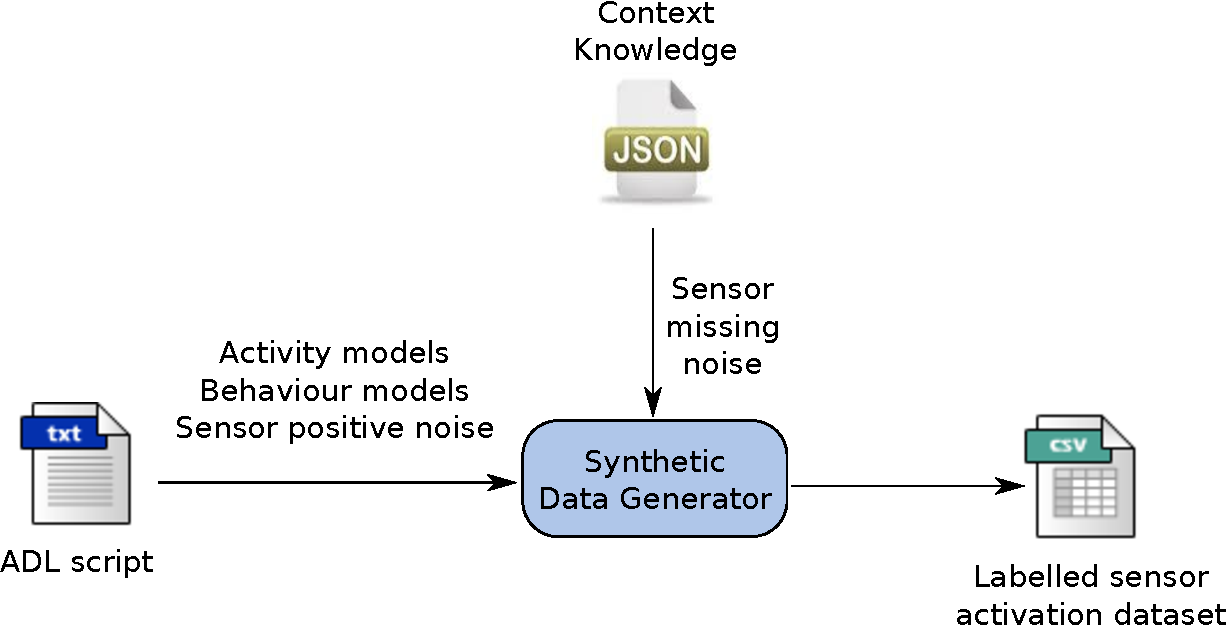
\includegraphics[width=\textwidth]{synthetic_tool.pdf}
    \caption{High-level design of the synthetic dataset generator tool.}
    \label{fig-synth-tool}
\end{figure}

The first part of the \textit{ADL script} is for defining \textit{sensor activation patterns} for activities. Sensor activation patterns are used to describe how activities are performed in terms of sensor activations. An activity can have an arbitrary number of sensor activation patterns, which are specified with an occurrence probability and a sequence of sensor activations with relative time lapses. An example of sensor activation patterns for activity \textit{MakeCoffee} can be found in Figure \ref{fig:sensor-act}.

\begin{figure}
\begin{small}
\lstset{linewidth=\textwidth}
\begin{lstlisting}
MakeCoffee 2
0.50 storeSens@0 mugSens@5 fridgeSens@10 smilkSens@5 
     afcoffeeSens@5 coffeePotSens@15 potSens@20 
     microwaveSens@20
0.50 storeSens@0 cupSens@5 fridgeSens@10 smilkSens@5 
     afcoffeeSens@5 coffeePotSens@15 potSens@20 
     microwaveSens@20
\end{lstlisting}
\end{small}
\caption{Sensor activation patterns for \textit{MakeCoffee} activity. The activity has two activation patterns with equal probability.}
\label{fig:sensor-act}
\end{figure}

The values that come after the '@' symbol represent the time in seconds between the previous sensor activation and the current one. The synthetic dataset generator establishes a time lapse with a Gaussian random generator whose mean value is the value specified in the script and the standard deviation is the 25\% of the mean. This way, time lapses between two consecutive sensor activations are realistic. 

The second part of the \textit{ADL script} defines the so called \textit{activity patterns}, which represent different days of the user in terms of performed activities. Two kinds of activity patterns are defined: (i) \textit{sequences}, where a time slot is given with a sequence of activities and time lapses between two consecutive activities, and (ii) \textit{alterations}, where a probability value is assigned to an activity to be performed in a concrete time slot. An example is depicted in Figure \ref{fig:activity-pattern}. A typical day of a user is described, with an occurrence probability of 0.29, since the activity pattern describes a weekend day ($2/7 \simeq 0.29$). In this case, the user reported that (s)he sometimes reads a book in the afternoon. Alterations allow modelling this kind of behaviour.


\begin{figure}
\begin{small}
\lstset{linewidth=\textwidth}
\begin{lstlisting}
Prob 0.29 4
S 9:00-10:00 MakeCoffee@0 BrushTeeth@1800 ReadBook@120
S 13:30-14:30 MakePasta@0 BrushTeeth@600
S 22:00-23:00 BrushTeeth@0 WashHands@10
A 18:00-20:00 ReadBook 0.5
\end{lstlisting}
\end{small}
\caption{An example of an activity pattern, which has an occurrence probability of 0.29 and it is composed of three sequences and an alteration.}
\label{fig:activity-pattern}
\end{figure}

The third part of the script is to define \textit{positive sensor noise}, which models the probability for a concrete sensor to get activated in an hour interval independently of ongoing activities. Positive sensor noise is used to model sensor errors and user's erratic behaviour. Erratic behaviour refers to user-object interactions that are not part of an activity. Imagine a user wants to prepare some pasta. Once the store has been open, to grab pasta a coffee recipient has to be moved. This interaction will be registered by the sensor attached to the coffee recipient, but it is not part of the activity. To model sensor positive noise, a probability is assigned to concrete sensors. Synthetic activity generator will use those probabilities to produce noise each hour, using a uniform probability distribution. 

But to model sensor errors, positive sensor noise is not enough. Sometimes, sensors that should get activated, fail. To model those errors another file is used: the context model file. This file is a \textit{Json}\footnote{http://www.json.org/} file where objects of the environment, attached sensors and sensor error models are defined. The file is used to acquire sensor error models, which in our case, have been obtained from the analysis given in \cite{Chen2012a}. Using this information, synthetic dataset generator introduces a failing probability to any sensor that has to be activated, achieving more realistic datasets. %Finally, the \textit{ADL script} contains the number of days to be simulated under those conditions. 

Using the \textit{ADL script} and the context model file, the synthetic dataset generator creates a CSV file where each sensor activation has an associated time-stamp and is labelled with an activity name or with special label \textit{None} if it is caused by noise. Additionally, activity start and end time are marked in the dataset.

\subsection{Discussion about the Hybrid Methodology}
%\label{sec:discussion}
\begin{comment}
- Explain the advantages: generate virtually infinite datasets, arbitrary number of days, perfectly labelled, sensor noise, erratic behaviour, realistic time lapses
 - Explain the main disadvantages: erratic behaviour difficult to capture
 \end{comment}
The methodology explained in Section \ref{sec:hybrid-approach} and implemented through Sections \ref{sec:survey} and \ref{sec:synthetic} has several advantages over the standard methodology explained in Section \ref{sec:introduction}. Let us enumerate and justify the advantages:

\begin{enumerate}
 \item The hybrid methodology is cheap and fast: it does not need to acquire or build any special environment, which can be an important investment. 
 \item A lot of users' information can be used: as it is based on surveys, it is generally easy to achieve a great number of users for the tests.
 \item Ethical and legal issues are much softer: in contrast with the standard methodology, there are no experiments with human beings. The only important point to be considered is the anonymity of users.
 \item Datasets can be generated on demand: using the synthetic dataset generator, arbitrary number of datasets can be generated as needed.
 \item Perfectly labelled datasets can be obtained: the synthetic dataset generator labels all sensor activations according to the given script and sensor error models. In consequence, the generated dataset is a perfect ground truth. 
 \item The influence of researchers is minimised: using surveys, researchers cannot write their own scripts with their bias. Even though researchers are still responsible of writing the scripts, following appropriate survey-script translation criteria, researchers' influence in the datasets is minimised.
 \item Any kind of scenarios can be implemented: the synthetic dataset generator allows preparing experiments where no sensor noise exist, where only a concrete kind of sensor noise exists or where conditions are as close as possible to realistic settings. The chance of implementing all those varieties of scenarios allows researchers test deeper their activity recognition systems, since they can see the influence of any factor they consider relevant. 
\end{enumerate}

However, there are some disadvantages also. For example, modelling user erratic behaviour is not easy. Although synthetic dataset generator offers a way to model this kind of interaction, it cannot capture it accurately. Another disadvantage refers to the information provided in surveys. Some users are very precise in their answers, but some are not. Sometimes, important details of activities are omitted by users in their answers, hence the precise way of performing activities cannot always be captured.